%----------------------------------------------------------------------------------------
%	PACKAGES AND OTHER DOCUMENT CONFIGURATIONS
%----------------------------------------------------------------------------------------
\documentclass[a4paper,12pt]{article}
\usepackage[english]{babel}
\usepackage[latin1]{inputenc}
\usepackage{amsmath}
\usepackage{xcolor}
\usepackage{amssymb}
\usepackage{amsfonts}
\usepackage{graphicx}
\usepackage{geometry}
\definecolor{link}{rgb}{0.4, 0.2, 0.2}
\geometry{
	a4paper,
	total={170mm,257mm},
	left=20mm,
	top=20mm,
}
\usepackage{hyperref}
\hypersetup{
	unicode=false,          % non-Latin characters in Acrobat’s bookmarks
	pdftoolbar=true,        % show Acrobat’s toolbar?
	pdfmenubar=true,        % show Acrobat’s menu?
	pdffitwindow=false,     % window fit to page when opened
	pdfstartview={FitH},    % fits the width of the page to the window
	pdftitle={Research Planning Report},    % title
	pdfauthor={Aaron Panaitescu},     % author
	pdfkeywords={neuroplasticity, Parkinson's, stimulation}, % list of keywords
	pdfnewwindow=true,      % links in new PDF window
	colorlinks=true,       % false: boxed links; true: colored links
	linkcolor=link,          % color of internal links (change box color with linkbordercolor)
	citecolor=link,        % color of links to bibliography
	filecolor=link,      % color of file links
	urlcolor=link           % color of external links
}
 
\usepackage{svg}
\usepackage{subcaption}
\usepackage{cleveref} 
\usepackage{float} 

\newcommand{\ballarrow}{\tikz[baseline=-0.6ex]{\draw[->] (0,0) -- (0.5,0); \filldraw (0.5,0) circle (2pt);}}
\newcommand{\Na}{$Na^+$\xspace}
\newcommand{\K}{$K^+$\xspace}
\newcommand{\Ca}{$Ca^{2+}$\xspace}
\hyphenpenalty=750
 
\newcounter{acronymcount}
\newcounter{currentacronym}

\newcommand{\printacronymsinline}{%
  \noindent
  \setcounter{acronymcount}{0}%
  \forglsentries[\acronymtype]{\thislabel}{\stepcounter{acronymcount}}%
  \ifnum\value{acronymcount}>0%
    \paragraph{Acronyms:}%
    \setcounter{currentacronym}{0}%
    \forglsentries[\acronymtype]{\thislabel}{%
      \stepcounter{currentacronym}%
      \glsentryshort{\thislabel} \glsentrydesc{\thislabel}%
      \ifnum\value{currentacronym}<\value{acronymcount}%
        , %
      \else
        .%
      \fi
    }%
  \fi
}

\newacronym{pd}{PD}{Parkinson's disease}
\newacronym{cbgt}{CBGT}{Cortico-Basal Ganglia-Thalamic}
\newacronym{snc}{SNc}{Substantia Nigra pars Compacta}
\newacronym{dbs}{DBS}{Deep brain stimulation}
\newacronym{adbs}{aDBS}{adaptive \acrshort{dbs}}
\newacronym{stn}{STN}{Subthalamic nucleus}
\newacronym{bg}{BG}{Basal ganglia} 
\newacronym{stdp}{STDP}{spike-timing-dependent plasticity}
\newacronym{gpe}{GPe}{Globus pallidus pars externa}
\newacronym{crs}{CRS}{Coordinated reset stimulation}
\newacronym{ap}{AP}{action potential}
\newacronym{if}{IF}{Integrate-And-Fire}
\newacronym{hh}{HH}{Hodgkin-Huxley}
\newacronym{lfp}{LFP}{local field potential}

\makeglossaries


\begin{document}
\begin{titlepage}
	\newcommand{\HRule}{\rule{\linewidth}{0.5mm}}
	\setlength{\topmargin}{0in}
	\center

	\begin{flushleft} \large
		\begin{minipage}{0.4\textwidth}
			
\includegraphics[scale=0.14]{imperial.png}
		\end{minipage}
	\end{flushleft}
	\vspace{4cm}

	%----------------------------------------------------------------------------------------
	%	TITLE SECTION
	%----------------------------------------------------------------------------------------
	\textbf{\large Literature review and thesis proposal}\\[0.1cm]
	{\large MRes. Neurotechonlogy}\\[0.5cm]

	\HRule \\[0.4cm]
	{\Large \bfseries Investigating plasticity in \\ Cortico-Basal Ganglia-Thalamus models \\ to improve stimulation-based treatments }
	\HRule \\[1cm]

	%----------------------------------------------------------------------------------------
	%	AUTHOR SECTION
	%----------------------------------------------------------------------------------------

	{\large Aaron Panaitescu \\
	(\textit{CID:} 02054726) \\[0.4cm]
	\textbf{Supervisor:} \\
	Dr. Hayriye Cagnan}

	%----------------------------------------------------------------------------------------
	%	DATE SECTION
	%----------------------------------------------------------------------------------------

	\vfill
	{Word Count: 1911}\\[0.4cm]
	{\large \today}\\[0.8cm]
\end{titlepage}
%----------------------------------------------------------------------------------------
%	REPORT CONTENT
%----------------------------------------------------------------------------------------
\pagenumbering{roman}
\tableofcontents
\vfill
\printacronymsinline

\newpage
\pagenumbering{arabic}
\setcounter{page}{1}

\section{Introduction}
\acrfull{pd} is characterised by pathological hypersynchrony in \acrfull{cbgt} circuit, driven by
dopaminergic degeneration in the \acrfull{snc}.
\acrlong{dbs} of the \acrfull{stn} alleviates tremor by disrupting
hypersynchrony in the \acrfull{bg}.
However, the mechanism through which this happens remains not well understood, and therapeutic effects are transient,
requiring continuous stimulation.
The goal of this study is to propose a computational framework to investigate multi-site phase-locked stimulation in a
spiking \acrshort{cbgt} network model with \acrfull{stdp} rules, aiming to induce lasting desynchronisation
through activity-dependent synaptic reorganisation.

Pathological and healthy network regimes will be established through data-driven tuning of spiking
neuron models.
Systematic simulations then evaluate multi-site phase-locked stimulation across three experimental axes:
(1) \acrshort{stdp} enabled/disabled in various \acrshort{cbgt} nuclei,
(2) stimulation applied to different pairs of basal ganglia populations and cortical afferents, and
(3) closed-loop adaptation to thalamic oscillatory activity.
The network will then be analysed in terms of the inter-populational coupling and the stability of potential
stimulation-driven non-pathological states.

This work advances the field in two key directions:
(1) integrates phase-locked stimulation with plasticity-targeted protocols, and
(2) evaluates stimulation targets across the \acrshort{cbgt} circuit focusing on regions with experimentally validated \acrshort{stdp}.
Results will inform clinical adaptive stimulation protocols that exploit neuroplasticity for lasting symptom relief,
while the methodology provides a generalisable computational framework for closed-loop neuromodulation design.

\section{Background and literature review}

\subsection{Parkinson's Disease}
\acrshort{pd} is characterised by the loss of dopaminergic neurons and the presence of
Lewy Bodies in the \acrshort{snc} \cite{del2018advances}. This dopaminergic depletion in the \acrshort{snc} leads to striatal dopamine
deficiency, which in turn leads to excessive synchronisation in the basal ganglia.
Hypersynchrony is a hallmark of the \acrshort{pd} \cite{hammond2007pathological, helmich2012cerebral},
and thus, can be a promising therapeutic target.


\subsection{Deep brain stimulation: theory and practice}
It is believed tremor originates from excessive coupling in the \acrshort{cbgt} network.
Thus, \acrshort{dbs} in this region emerged as an effective tool in treating advanced \acrshort{pd} and Essential tremor
patients \cite{del2018advances}.
\acrshort{dbs} works by delivering high-frequency stimulation in regions of the \acrshort{cbgt}
through implanted electrodes.
A prominent theory for this method's success is that it enables stimulation-driven
decorrelation of the different \acrshort{bg} nuclei, shifting it to a non-pathological state.
There is significant evidence that performing \acrshort{dbs} in the \acrshort{stn} or the GPi can have significant improvements in
quality of life in patients, reducing tremor and restoring motor control
\cite{rodriguez2005bilateral, rubin2004high}.

However, \acrshort{dbs} does have significant limitations. Firstly, like any highly invasive procedure, the implantation procedure has many risks.
Advances in electrode technology and surgical techniques have reduced some of these risks *cite*.
Secondly, patient symptoms are only ameliorated while the stimulation is on. This means that
the device needs to be on continuously, which can induce numerous side effects in patients
**citeee** and also creates the need for a continuous power supply.
Finally, the mechanism through which \acrshort{dbs} reduces tremors is not fully understood yet.
For instance, there is a discrepancy in tremor frequency ($\sim$ 20 Hz on average) and the effective frequency range of
traditional \acrshort{dbs} of 130-180 Hz.

Therefore, several areas of research emerge in improving stimulation-based treatments of \acrshort{pd}:
finding non-invasive alternatives \cite{saturnino2017target, schwab2020spike}, eliciting lasting,
plastic changes in the \acrshort{cbgt} circuit, closing the loop and coupling stimulation to the presence of
patient symptoms (\acrfull{adbs}, \cite{beudel2018adaptive}), and phase-locking stimulation to
rythmic activity in the \acrshort{cbgt} \cite{cagnan2017stimulating, west2022stimulating}.

\begin{figure}[ht]
	\centering
	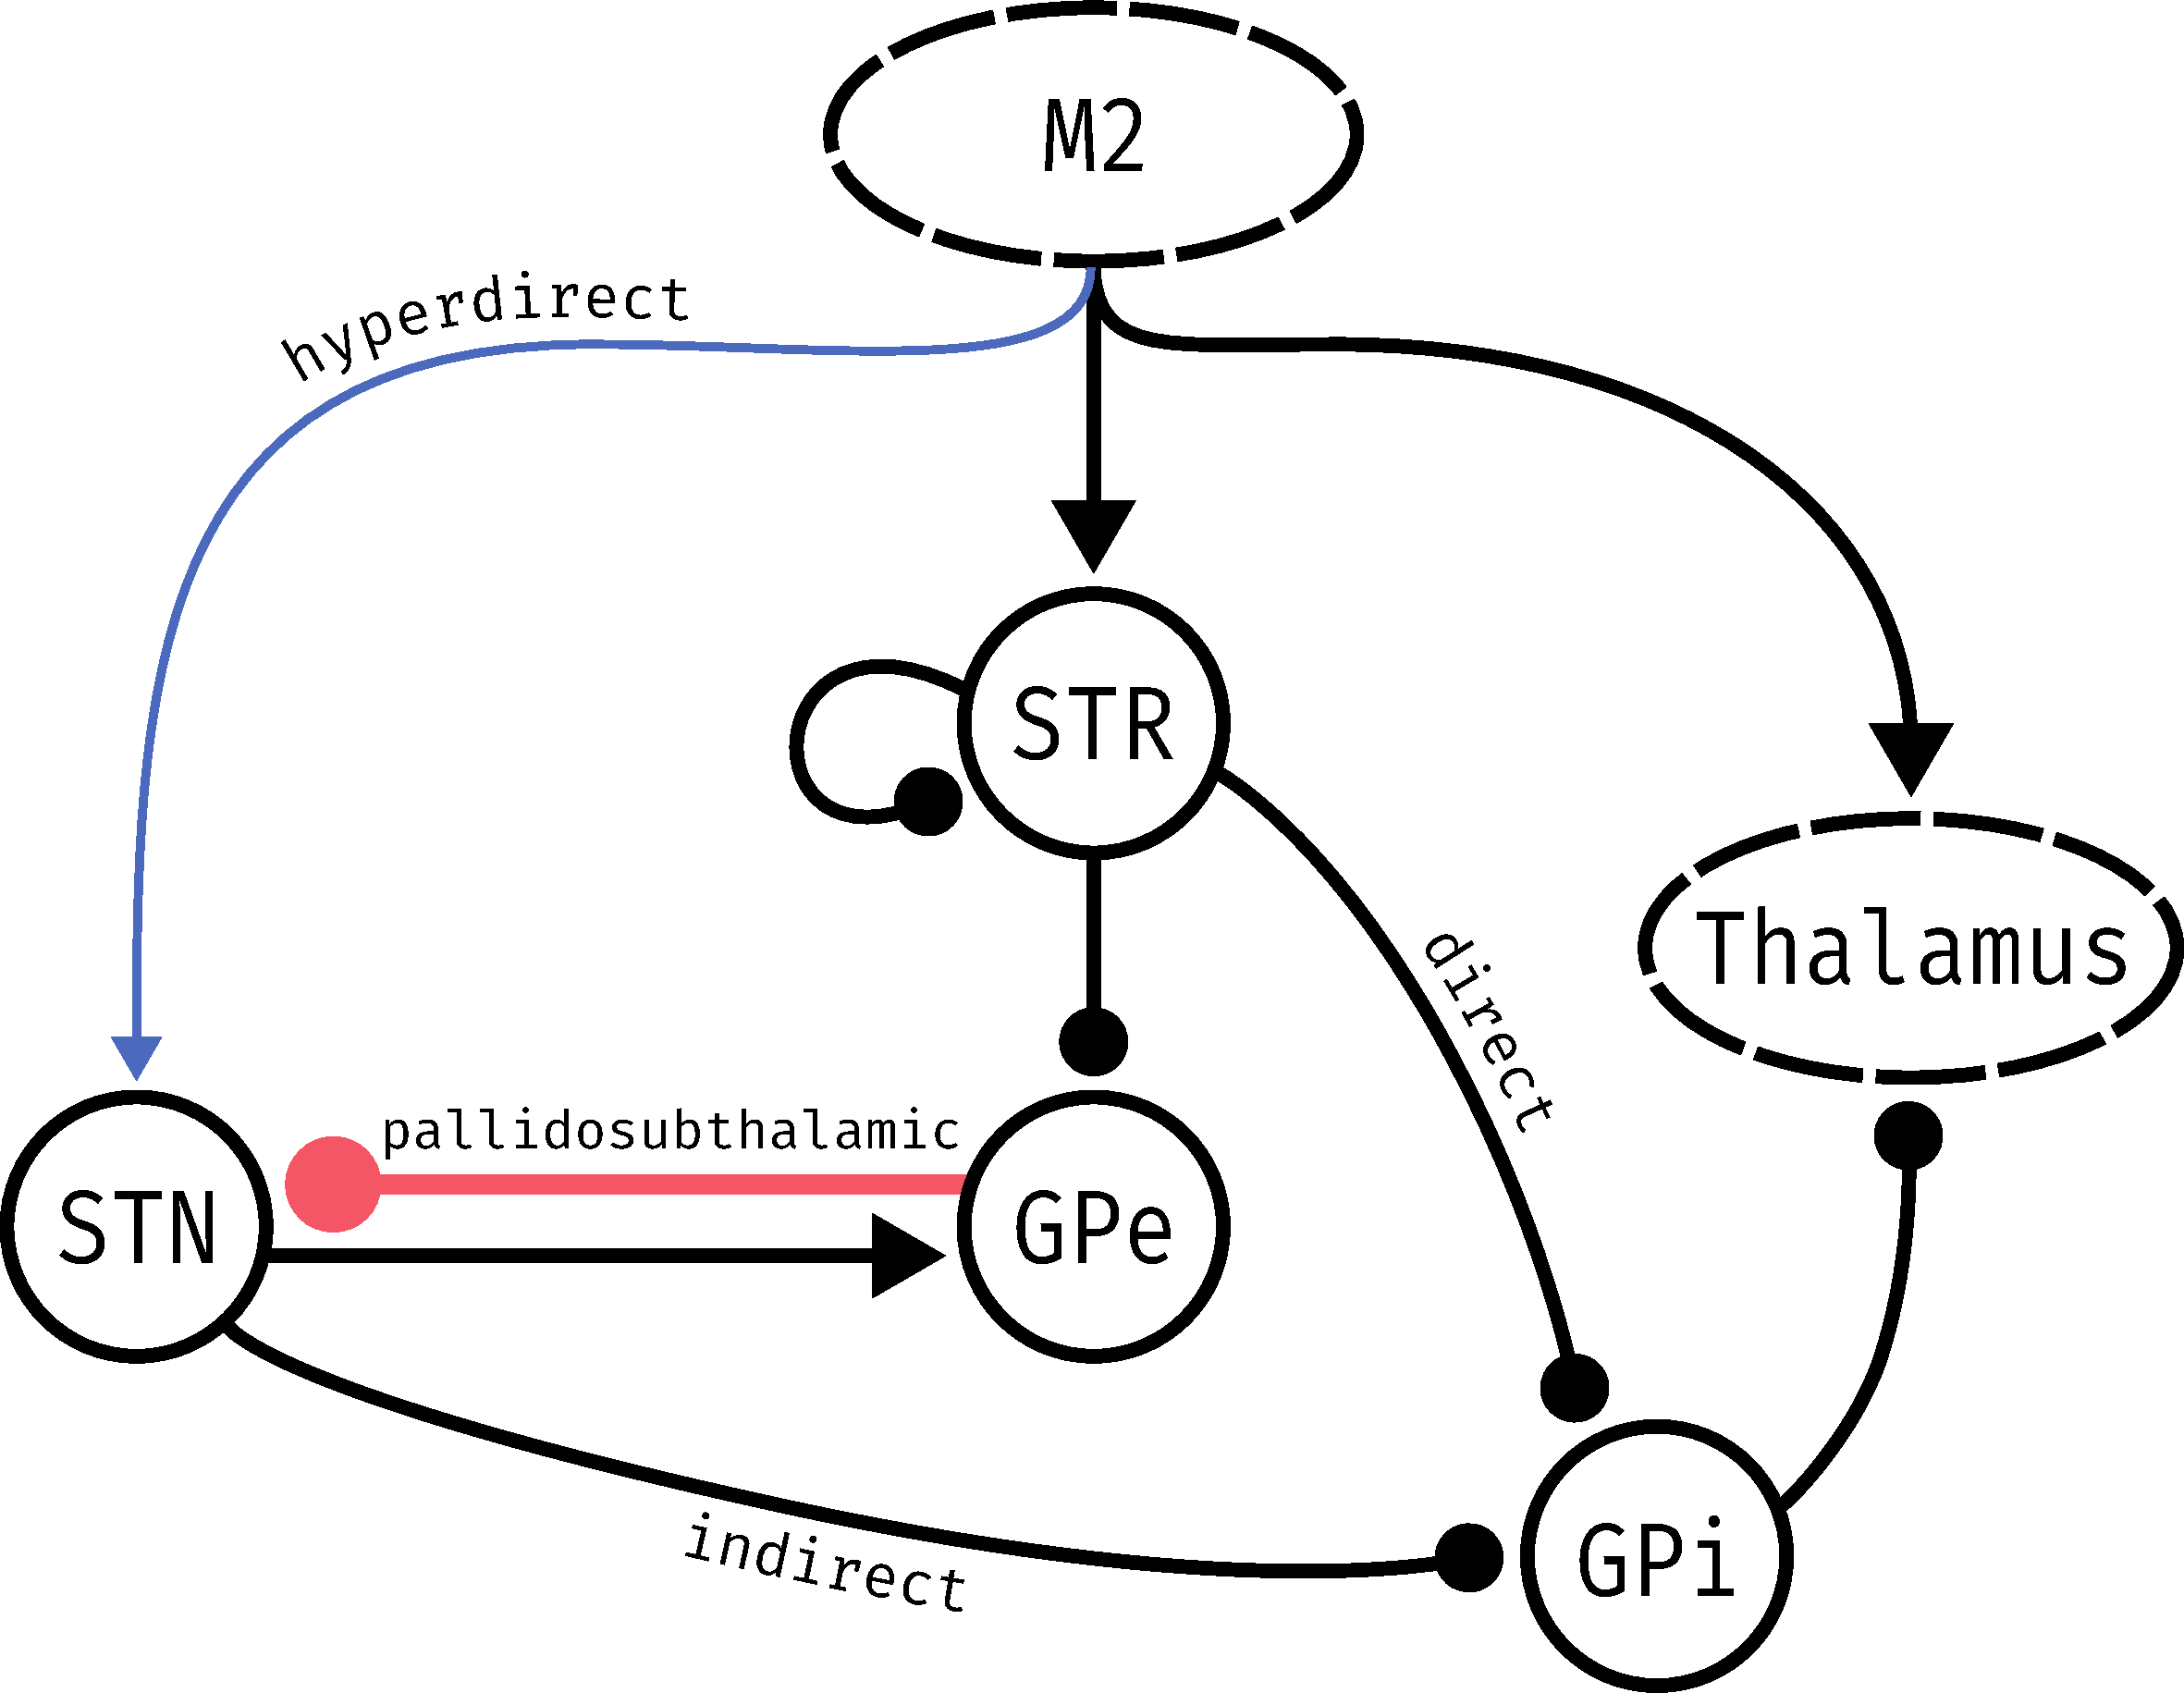
\includegraphics[width=0.6\textwidth]{figs/cbgt_circuit.pdf}
	\caption{\acrshort{cbgt} circuit in \acrshort{pd} pathology. Arrow connections represent majority excitatory (glutamate) connections,
		ball arrows represent inhibitory (GABA) connections.}
\end{figure}

\subsection{Stimulating at the right time}
The parkinsonian state results from the complex interplay between four pathways in the \acrshort{cbgt}
the \textbf{hyperdirect} excitatory cortico-subthalamic pathway,
the \textbf{direct} inhibitory striatopallidal pathway,
the \textbf{indirect} inhibitory subthalamopallidal pathway and
the inhibitory \textbf{pallidosubthalamic} (PS) pathway. In pathology the hyperdirect
pathway is downregulated, while the PS pathway is upregulated, leading to a shift in
beta-band oscillatory activity from sub-band $\beta_1$ to sub-band $\beta_2$, which correlates to
hypersynchrony in the basal ganglia \cite{west2022stimulating}.

\cite{cagnan2017stimulating} demonstrated that phase-specific neuromodulation can disrupt pathological
synchrony in essential tremor by delivering stimulation pulses locked to thalamic oscillatory phases.
Strategies like this and others (e.g., \acrshort{adbs} \cite{beudel2018adaptive}) show the potential for closed-loop,
adaptive therapies to address hypersynchrony in the \acrshort{bg}.

\subsection{Plasticity to recover network states}
Neuroplasticity can be defined as "the ability of the nervous system to change its activity in
response to intrinsic or extrinsic stimuli by reorganising its structure, functions, or
connections" \cite{mateos2019impact}.
Plasticity occurs at different scales in the brain, ranging from molecular to neural networks.
The focus of this project is synaptic plasticity, which occurs between a pre-synaptic and a
post-synaptic neuron. The mechanisms of plasticity have been thoroughly studied **cite**, and
are starting to find their way into clinical applications in neurorehabilitation (e.g., stroke, trauma,
spinal cord injury \cite{cramer2011harnessing}) and neuroprostheses \cite{lebedev2017brain}.

The potential of plasticity-based treatments in \acrshort{pd} depends on the existence of
spike-timing-dependent plasticity (\acrshort{stdp}) in the synapses of the different \acrshort{bg} nuclei, particularly
in the \acrshort{stn} \cite{rubin2012basal}. Long and short-term plasticity has been found in
corticostriatal synapses \cite{kreitzer2008striatal, di2009short} as well as cell-specific \acrshort{stdp} in
striatal interneurons \cite{fino2010spike}.
\cite{thieu2024role} modelled \acrshort{stdp} and random inputs in \acrshort{stn} neuronal population and found combining the two can
increase coupling between neurons.

To exploit \acrshort{stdp} in the \acrshort{cbgt}, \acrfull{crs} has been proposed by Hauptmann and Tass.
\acrshort{crs} delivers brief, phase-targeted electrical stimuli to specific neuronal subpopulations within interconnected
neural circuits.
\acrshort{crs} has been computationally modelled in a \acrfull{gpe}-\acrshort{stn} network to successfully disrupt pathological
synchronisation in the \acrshort{bg} \cite{hauptmann2009cumulative, hauptmann2010restoration}.

\subsection{Modeling neural networks}
Most neuronal dynamics models are defined by rules of how voltage in a unit changes
over time in response to voltage in the network and external current (e.g., noise, stimulation
current).
This raises the question: what is a unit? From this two broad categories emerge: A unit can be an individual neuron or a cluster of neurons. This section introduces
some common types of models, justifying the direction chosen for this project.

\paragraph{Spiking neuron models} work by combining networks of units that individually
simulate neuronal \acrlong{ap}s (\acrshort{ap}s).
These networks can then be organised into different nuclei (e.g., \acrshort{stn}) and coerced to respect
excitatory or inhibitory connections between nuclei.
Within this class of models, different schemes for modelling neuronal dynamics exist,
such as \acrfull{if} \cite{gerstner2014if} and Hodgkin-Huxley
\cite{hodgkin1952measurement, gerstner2014hh}.

\paragraph{Mean-field models} simulate the \acrlong{lfp}s (\acrshort{lfp}s) of clusters of neurons
and connect these clusters with population-level connectivity rules. (e.g.,
\cite{jansen1995electroencephalogram, west2022stimulating})

% Neuron-level
\subsubsection{Integrate-And-Fire}
\begin{figure*}[ht]
	\centering
	\begin{subfigure}[t]{0.48\textwidth}
		\centering
		\caption{}
		\includesvg[height=1.4in]{figs/ifu}
		\label{fig:ifu}
	\end{subfigure}
	~
	\begin{subfigure}[t]{0.48\textwidth}
		\centering
		\caption{}
		\includesvg[height=1.4in]{figs/ifi}
	\end{subfigure}
	\caption{(a) Voltage trace of IF unit overtime in response to external current in (b). When the potential crosses
		the AP threshold it is reset and the spike is recorded.}
	\label{fig:if}
\end{figure*}

\acrshort{if} models treat action potentials as events.
This reduction is justified by the fact that the shape of \acrshort{ap}s is always \textit{approximately}
the same, meaning they \textit{cannot} convey information. \cite{gerstner2014if} describe a leaky \acrshort{if} model
is represented by an electrical circuit with a resistor($R$) and a capacitor($C$) in parallel
($I(t) = I_R + I_C$), combined with a reset condition when the potential exceeds a threshold
$\theta$ (\cref{fig:ifu}).
This can be modelled by,
\begin{align}
	\tau_m \dot u                                           & = -[u(t) - u_{rest}] + RI(t),                                    \\
	\intertext{Together with the reset condition,}
	\lim_{\delta \rightarrow 0; \delta > 0} u(t^f + \delta) & = u_r,                                                           \\
	t^f                                                     & = \{t | u(t)                                        = \theta \}.
\end{align}
Where $u$ is the membrane voltage, $u_{rest}$ is the resting potential, $u_r$ is the reset
potential, $\tau_m = RC$ is the time constant, and $I$ is external current.

These equations describe the update rules in a single unit. Connectivity rules between units
can be added to form neural networks. These connections can then be strengthened or weakened
depending on spike timings between units, modelling \acrshort{stdp}. \cite{shupe2021integrate} simulate
plasticity in cortical columns; \cite{kromer2023synaptic} model plasticity between basal ganglia
nuclei both using an \acrshort{if} model.

\subsubsection{Hodgkin-Huxley}

\begin{figure*}[ht]
	\centering
	\includesvg[height=1.4in]{figs/hhu}
	\caption{Voltage trace of HH unit in response to external current pulses.}
	\label{fig:hh}
\end{figure*}

The \acrfull{hh} model \cite{hodgkin1952measurement} simulates membrane potential by
considering the dynamics of different ion conductances.
Each ion has a reversal potential at which the force of the electrical and chemical gradients
across the membrane even out.
These can be modeled in an electrical circuit as a battery and the total channels of a
particular ion can be modeled as a resistor. Each modelled ion has a parallel branch in the
corresponding electrical circuit. The following equations adapted from \cite{gerstner2014hh}
describe the \acrshort{hh} model:
\begin{align}
	I(t) & = I_C(t) + \sum_k I_k(t),
	\intertext{Where the current of each ion $k$ can be described in terms of the open probability
		of a $k$ channel, $p_k$ and the maximum conductance when all $k$ channels are open, $g_k$:}
	I_k  & = g_k p_k(u - E_k).
\end{align}
In particular Hodgkin and Huxley modeled $Na^+$, $K^+$ and a leak $L$ currents:
\begin{align}
	C \dot u = g_{Na}m^3h(E_{Na} - u) + g_K n^4(E_K - u) + g_L (E_L - u),
\end{align}
Where $m$, $h$ and $n$ are open probabilities for subunints of $Na$ or $K$ channels governed by:
\begin{align}
	\dot x = - \frac 1 {\tau_m(u)}[x - x_0(u)], &  & x \in \{m, h, n\}.
\end{align}
As in the \acrshort{if} model, these rules describe the dynamics of a single unit, which can subsequently
be connected to model a network of neurons (e.g., \cite{terman2002activity}) and augmented to
include plasticity rules \cite{borges2016effects}.

\subsubsection{Rubin-Terman}
\cite{terman2002activity} augmented the \acrshort{hh} model to create a subthalamopallido network of the
basal ganglia (RT model), where \acrshort{gpe} and \acrshort{stn} neurons are modelled according to the following equation,
\begin{align}
	C \dot u = - I_L - I_K - I_{Na} - I_T - I_{Ca} - I_{AHP} - I_{s \rightarrow d} -
	I_{s \rightarrow s} + I_{app}
\end{align}
Where leak ($L$), \K, \Na and high-threshold \Ca currents \cite{song2000characterization}, are
described in \acrshort{hh}-like equations, and low threshold calcium current $I_T$ is different for \acrshort{gpe} and
\acrshort{stn} neurons. $I_{AHP}$ represents \Ca-activated, voltage-independent \textit{afterhyperpolarisation}
(AHP) $K^+$ current. $I_{s \rightarrow d}$ represents the inter-populational influence and is
defined by
$I_{s \rightarrow d} = \sum_{j} I_{ij}^{ds}$ where $s, d \in \{\text{\acrshort{gpe}}, \text{\acrshort{stn}}\}$.
$I_{ij}^{ds}$ is the current from the presynaptic neuron $j$ in $s$ to the
postsynaptic neuron $i$ in $d$, and is defined by
$I_{ij}^{ds} = w_{ij}^{ds}s_{ij}^{ds}(t - \tau_{ds})(u_i - E_{ds})$ where $w_{ij}$ is the
synaptic strength, $s_{ij}^{ds}$ is a synaptic variable and $\tau_{ds}$ is the transmission
delay between $d$ and $s$.
\cite{madadi2022inhibitory} expand on this model by adding inhibitory spike-timing-dependent
plasticity to this network with $\Delta w = \eta(\exp(-|\Delta t| / \tau_w) - \alpha)$,
where $\eta$ is the \textit{learning rate}, $\tau_w$ is the time constant of the plasticity
rule exponential decay and $\alpha$ is the depression factor.

% Population
\subsubsection{Other modeling approaches}
Neuronal populations can also be modelled with networks of coupled phase-oscillators as in
\cite{tass2006long}. \cite{duchet2023mean} modelled \acrshort{stdp} as mean-field phase-locked plasticity in a network of
Kuramoto oscillators \cite{kuramoto1984phase}. In the context of this project studying phase-locked stimulation
to exploit phase-dependent plasticity rules would bias the experiments to non-null results.

\cite{jansen1995electroencephalogram} model cortical columns of neurons by considering the PSPs of
excitatory and inhibitory populations in a column to replicate EEG-recorded alpha and beta activity.
\cite{west2022stimulating} used these building blocks in a full \acrshort{cbgt} model to study the effects of
phase-dependent stimulation on coupling. Since these approaches work with \acrshort{lfp}s, plasticity
rules would have to be phase-dependent, so they would introduce the same issue as phase-oscillator networks.

\section{Project Plan}
The primary objective of this project is to investigate multi-site phase-locked stimulation in a spiking \acrshort{cbgt} network
model, with the goal of inducing plastic changes that transition pathological network dynamics of the \acrshort{bg} toward
a healthy desynchronised state. This work will address two important gaps in the current literature:
\begin{enumerate}[nosep]
	\item Integrating phase-locked stimulation with plasticity-targeted protocols, closing the loop in coordinated
	      reset paradigms.
	\item Systematically evaluating stimulation targets across the wider \acrshort{cbgt} network, with emphasis on regions with
	      experimentally validated synaptic plasticity (e.g., corticostriatal connections) while accounting for
	      uncertainties in plasticity mechanisms at other nodes like the \acrshort{stn}.
\end{enumerate}
The selection of a spiking network with \acrshort{stdp} rules over phase-oscillator models with phase-dependent plasticity is
motivated by the following methodological consideration:
Simulating phase-locked stimulation within systems governed by \textit{a priori} phase-triggered plasticity introduces
inherent circularity.
Such coupling risks conflating stimulation mechanisms with network adaptation rules, effectively predetermining
intervention outcomes without much dependence on physiological constraints.
In contrast, spiking networks with \acrshort{stdp} decouple the synchronisation mechanism from the phase-locked stimulation
preserving the causal distinction between stimulation protocols and plasticity-driven reorganisation.

\subsection{Methodology}
To achieve these objectives, the following steps are outlined:
\begin{enumerate}[nosep]
	\item Implement \acrshort{stdp} mechanisms within a spiking \acrshort{cbgt} network model.
	\item Tune pathological and healthy dynamical modes through data-driven parameter tuning, initially with plasticity disabled.
	\item Conduct systematic simulations of multi-site phase-locked stimulation under different experimental conditions:
	      \begin{enumerate}[nosep, label=\alph*.]
		      \item \acrshort{stdp} enabled or disabled in specific network nodes
		      \item Multi-site phase-locked stimulation applied to distinct \acrshort{bg} nuclei and cortical afferents
	      \end{enumerate}
	      Quantify network responses by analysing inter-nuclei coupling, and transitions between dynamical states.
	\item Derive stimulation protocols optimised for plasticity-driven network desynchronisation.
\end{enumerate}

\subsection{Timeline}
**Gant chart thingy**


%**********************************************%
\newpage
%----------------------------------------------------------------------------------------
%	REFERENCES
%----------------------------------------------------------------------------------------
\addcontentsline{toc}{section}{References}
\bibliography{refs}
\bibliographystyle{apalike}
\newpage

%----------------------------------------------------------------------------------------
%	APPENDIX  
%----------------------------------------------------------------------------------------
\appendix
\section*{Appendices}
\addcontentsline{toc}{section}{Appendices}
\renewcommand{\thesubsection}{\Alph{subsection}}
\subsection{Research gap diagram}
\begin{figure}[ht]
	\centering
	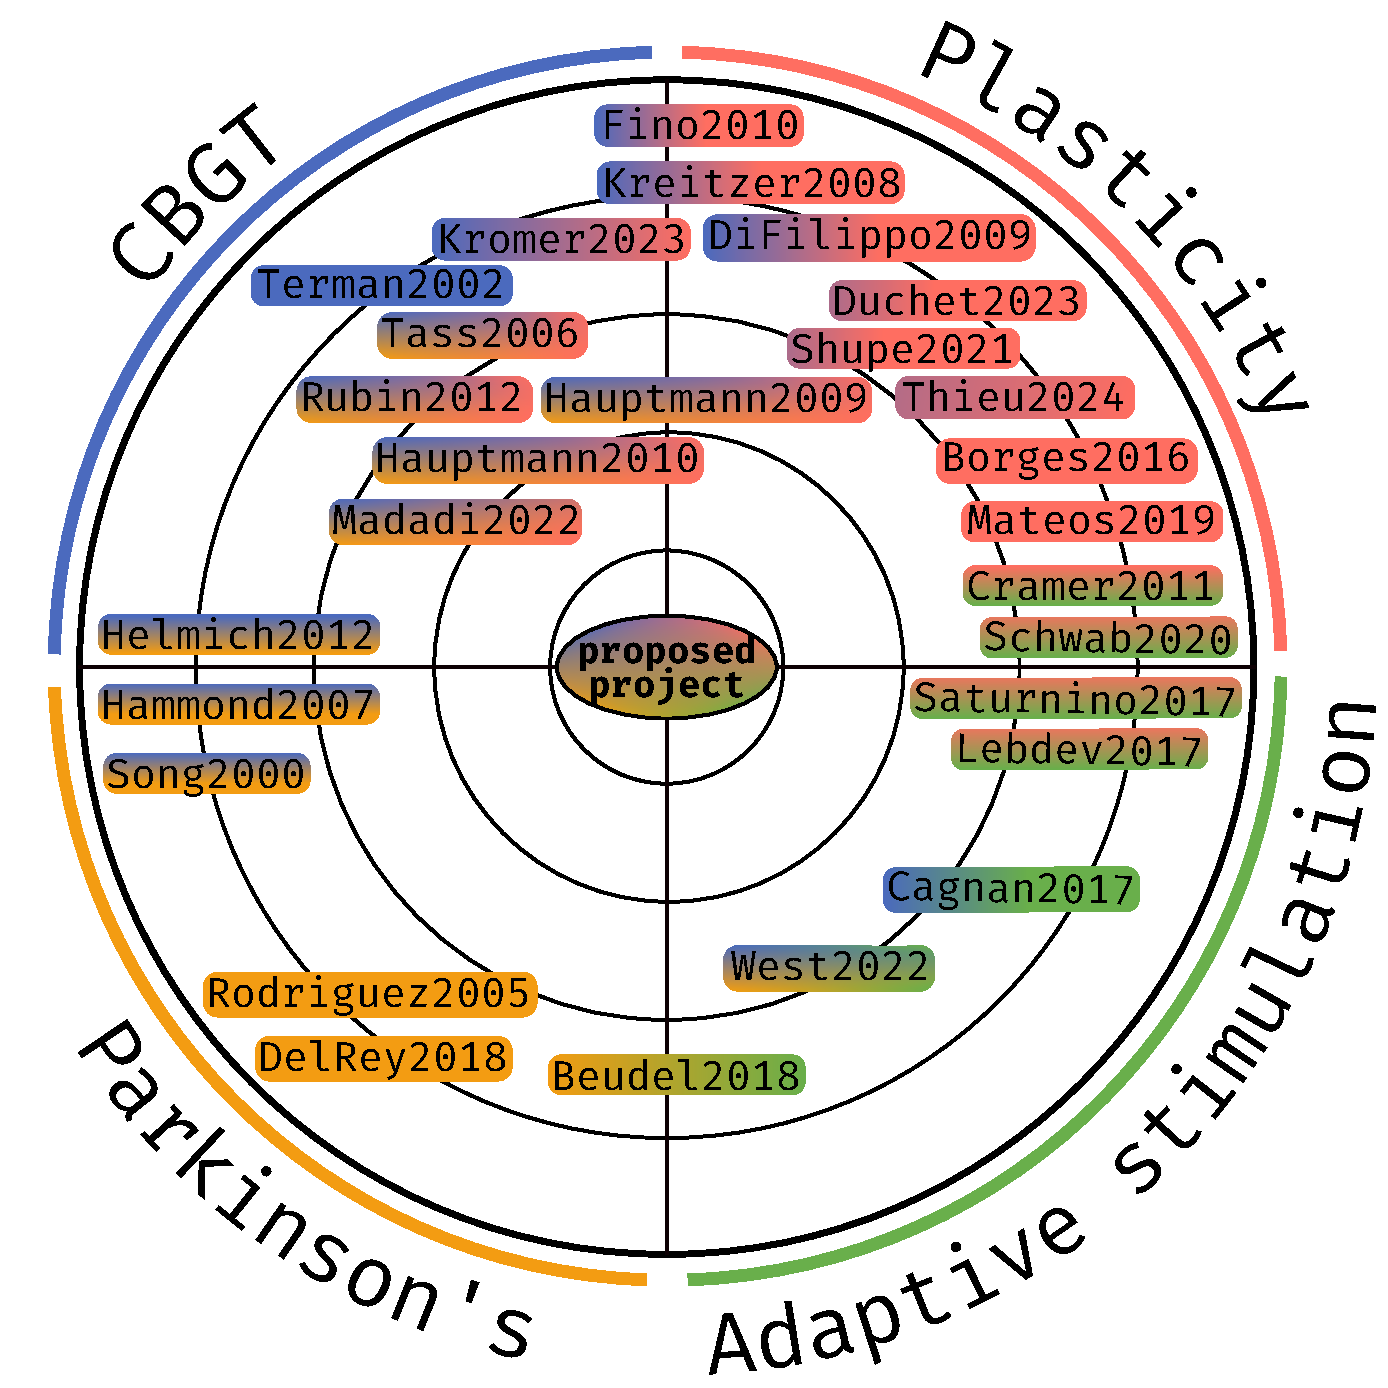
\includegraphics[width=0.6\textwidth]{figs/lit_diagram.pdf}
	\caption{Visulaisation of the targeted research gap.}
\end{figure}

\subsection{Report data}
The code used to generate \cref{fig:if,fig:hh} along with all the figures used in this report, are uploaded on GitHub at
\url{https://github.com/NemoInfo/NeuroModelSandbox} and \\
\url{https://github.com/NemoInfo/plasticity}


\end{document}
